\subsection{Stream Summarization}
\begin{frame}{Stream Summarization}


 \begin{center}
   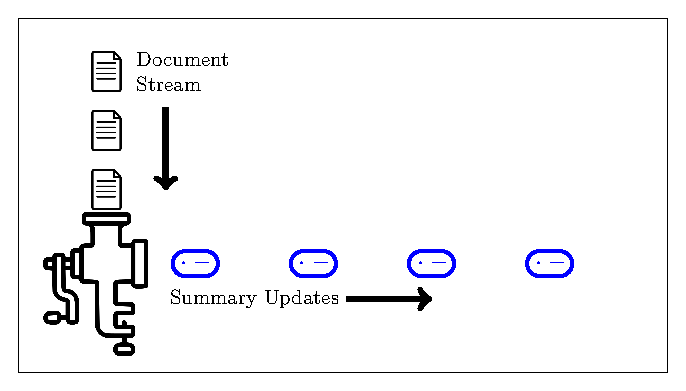
\includegraphics[scale=.8]{2_feature_based_models_of_salience/image_texs/stream_sum/stream_sum.pdf}
 \end{center}

 \begin{itemize}
     \item Data from \textbf{TREC Temporal Summarization Track}, 2013-2015
     \item \textbf{Query focused} crisis monitoring scenario 
  \item E.g., summarize a stream of news about Hurricane Sandy
 \end{itemize}
\end{frame}


%\begin{frame}
%    \begin{itemize}
%        \item When I was sixteen I dated a boy.
%        \item with my own name!
%        \item It was weird, moaining my own name,
%        \item while trying to \@\#?\$!
%\end{frame}


\begin{frame}{TREC Temporal Summarization Data}
  \begin{itemize}
      \item \alert<2>{\textbf{Stream Corpus}} (Document Stream Input)
    \begin{itemize}
      \item Timestapped collection of news websites.
      \item Simulates web news publishing.
    \end{itemize}
    \item \alert<3>{\textbf{Event Queries}} (Summarizer Focus)
    \begin{itemize}
      \item Queries correspond to real-life disasters/crises.
      \item E.g. ``Hurricane Sandy,'' or ``Boston Marathon Bombing''
    \end{itemize}
    \item \alert<4>{\textbf{Event Nuggets}} (Reference ``Summary'' atoms)
    \begin{itemize}
      \item Timestamped text snippets of important event facts.
      \item Selected by NIST from Wikipedia event page.
    \end{itemize}
  \end{itemize}

%No reference summaries, but reference \textit{nuggets}: ~\\
~\\

        \begin{tabular}{l}
         \textbf{Nuggets for event query ``hurricane sandy''} \\
        \hline
    $[\textrm{10/23 ~8:20pm}]$ Sandy strengthened from a tropical depression into\\
    ~~~~~~~~~~~~~~~~~~~~~~a tropical storm \\
    $[\textrm{10/23 ~8:20pm}]$ 2 pm Oct 23 Sandy moving north-northeast at 4 
    knots \\
    $[\textrm{10/23 ~8:53pm}]$ forecast track uncertain \\
    $[\textrm{10/25 12:20am}]$ In Jamaica damage was extensive\\
\end{tabular}

\end{frame}

%\begin{frame}{Sentence Salience for Stream Summarization} 
% \begin{itemize}
%    \item Let $S(q)$ be the ordered sequence of sentences from the relevant 
%        document stream for query $q$. ~\\~\\
%   \item Let $\mathcal{N}(q)$ be the set of nuggets for query $q$. ~\\~\\
%   \item \textbf{Salience} $y$ of a sentence $s\in S(q)$ is computed:  \[y = \max_{n \in \mathcal{N}(q)} 
%       \textsc{Similarity}(s,\only<1>{n}\only<2>{\alert{\cancel{n}}})\]  where $\textsc{Similarity}(\cdot, \cdot)$
%      is the semantic similarity method of Guo and Diab, 2012.~\\~\\
%\item<2>{\alert{No nugget knowledge at test time. Learn to predict $p(\hat{y}|s,q)$. }}
%    \end{itemize}
%\end{frame}
